% Options for packages loaded elsewhere
\PassOptionsToPackage{unicode}{hyperref}
\PassOptionsToPackage{hyphens}{url}
\PassOptionsToPackage{dvipsnames,svgnames,x11names}{xcolor}
%
\documentclass[
  12pt,
  a4paper, oneside]{starmastarticle}

\usepackage{amsmath,amssymb}
\usepackage{lmodern}
\usepackage{iftex}
\ifPDFTeX
  \usepackage[T1]{fontenc}
  \usepackage[utf8]{inputenc}
  \usepackage{textcomp} % provide euro and other symbols
\else % if luatex or xetex
  \usepackage{unicode-math}
  \defaultfontfeatures{Scale=MatchLowercase}
  \defaultfontfeatures[\rmfamily]{Ligatures=TeX,Scale=1}
\fi
% Use upquote if available, for straight quotes in verbatim environments
\IfFileExists{upquote.sty}{\usepackage{upquote}}{}
\IfFileExists{microtype.sty}{% use microtype if available
  \usepackage[]{microtype}
  \UseMicrotypeSet[protrusion]{basicmath} % disable protrusion for tt fonts
}{}
\makeatletter
\@ifundefined{KOMAClassName}{% if non-KOMA class
  \IfFileExists{parskip.sty}{%
    \usepackage{parskip}
  }{% else
    \setlength{\parindent}{0pt}
    \setlength{\parskip}{6pt plus 2pt minus 1pt}}
}{% if KOMA class
  \KOMAoptions{parskip=half}}
\makeatother
\usepackage{xcolor}
\usepackage[top=25mm,left=25mm,right=25mm,bottom=25mm]{geometry}
\setlength{\emergencystretch}{3em} % prevent overfull lines
\setcounter{secnumdepth}{-\maxdimen} % remove section numbering
% Make \paragraph and \subparagraph free-standing
\ifx\paragraph\undefined\else
  \let\oldparagraph\paragraph
  \renewcommand{\paragraph}[1]{\oldparagraph{#1}\mbox{}}
\fi
\ifx\subparagraph\undefined\else
  \let\oldsubparagraph\subparagraph
  \renewcommand{\subparagraph}[1]{\oldsubparagraph{#1}\mbox{}}
\fi


\providecommand{\tightlist}{%
  \setlength{\itemsep}{0pt}\setlength{\parskip}{0pt}}\usepackage{longtable,booktabs,array}
\usepackage{calc} % for calculating minipage widths
% Correct order of tables after \paragraph or \subparagraph
\usepackage{etoolbox}
\makeatletter
\patchcmd\longtable{\par}{\if@noskipsec\mbox{}\fi\par}{}{}
\makeatother
% Allow footnotes in longtable head/foot
\IfFileExists{footnotehyper.sty}{\usepackage{footnotehyper}}{\usepackage{footnote}}
\makesavenoteenv{longtable}
\usepackage{graphicx}
\makeatletter
\def\maxwidth{\ifdim\Gin@nat@width>\linewidth\linewidth\else\Gin@nat@width\fi}
\def\maxheight{\ifdim\Gin@nat@height>\textheight\textheight\else\Gin@nat@height\fi}
\makeatother
% Scale images if necessary, so that they will not overflow the page
% margins by default, and it is still possible to overwrite the defaults
% using explicit options in \includegraphics[width, height, ...]{}
\setkeys{Gin}{width=\maxwidth,height=\maxheight,keepaspectratio}
% Set default figure placement to htbp
\makeatletter
\def\fps@figure{htbp}
\makeatother

\usepackage{setspace}
\renewcommand{\familydefault}{cmss}
\renewcommand{\familydefault}{\sfdefault}
\usepackage{multirow}
\usepackage{colortbl}
\usepackage{fancyhdr}
\onehalfspacing
\renewcommand{\arraystretch}{1.2}
\setlength{\parskip}{0.5em}
\setlength{\parindent}{0em}
\newcommand{\mb}[1]{\mathbb{#1}} % blackboard bold
\newcommand{\mc}[1]{\mathcal{#1}} % calligraphic
\newcommand{\mf}[1]{\mathfrak{#1}} % fraktur
\newcommand{\ms}[1]{\mathscr{#1}} % script
\newcommand{\vb}[1]{\mathbf{#1}} % vector bold
\newcommand{\from}{\leftarrow}
\newcommand{\dne}{\hfill \qed \vspace{0.3cm}} % end of proof symbol
\newcommand{\abs}[1]{\left|#1\right|} % modulus signs
\newcommand{\norm}[1]{\left|\left|#1\right|\right|} % norm signs
\renewcommand{\Re}{\mathrm{Re}}
\renewcommand{\Im}{\mathrm{Im}}
\newcommand{\im}{\mathrm{im}}
\newcommand{\ds}{\displaystyle}
\makeatletter
\@ifpackageloaded{tcolorbox}{}{\usepackage[many]{tcolorbox}}
\@ifpackageloaded{fontawesome5}{}{\usepackage{fontawesome5}}
\definecolor{quarto-callout-color}{HTML}{909090}
\definecolor{quarto-callout-note-color}{HTML}{0758E5}
\definecolor{quarto-callout-important-color}{HTML}{CC1914}
\definecolor{quarto-callout-warning-color}{HTML}{EB9113}
\definecolor{quarto-callout-tip-color}{HTML}{00A047}
\definecolor{quarto-callout-caution-color}{HTML}{FC5300}
\definecolor{quarto-callout-color-frame}{HTML}{acacac}
\definecolor{quarto-callout-note-color-frame}{HTML}{4582ec}
\definecolor{quarto-callout-important-color-frame}{HTML}{d9534f}
\definecolor{quarto-callout-warning-color-frame}{HTML}{f0ad4e}
\definecolor{quarto-callout-tip-color-frame}{HTML}{02b875}
\definecolor{quarto-callout-caution-color-frame}{HTML}{fd7e14}
\makeatother
\makeatletter
\makeatother
\makeatletter
\makeatother
\makeatletter
\@ifpackageloaded{caption}{}{\usepackage{caption}}
\AtBeginDocument{%
\ifdefined\contentsname
  \renewcommand*\contentsname{Table of contents}
\else
  \newcommand\contentsname{Table of contents}
\fi
\ifdefined\listfigurename
  \renewcommand*\listfigurename{List of Figures}
\else
  \newcommand\listfigurename{List of Figures}
\fi
\ifdefined\listtablename
  \renewcommand*\listtablename{List of Tables}
\else
  \newcommand\listtablename{List of Tables}
\fi
\ifdefined\figurename
  \renewcommand*\figurename{Figure}
\else
  \newcommand\figurename{Figure}
\fi
\ifdefined\tablename
  \renewcommand*\tablename{Table}
\else
  \newcommand\tablename{Table}
\fi
}
\@ifpackageloaded{float}{}{\usepackage{float}}
\floatstyle{ruled}
\@ifundefined{c@chapter}{\newfloat{codelisting}{h}{lop}}{\newfloat{codelisting}{h}{lop}[chapter]}
\floatname{codelisting}{Listing}
\newcommand*\listoflistings{\listof{codelisting}{List of Listings}}
\makeatother
\makeatletter
\@ifpackageloaded{caption}{}{\usepackage{caption}}
\@ifpackageloaded{subcaption}{}{\usepackage{subcaption}}
\makeatother
\makeatletter
\@ifpackageloaded{tcolorbox}{}{\usepackage[many]{tcolorbox}}
\makeatother
\makeatletter
\@ifundefined{shadecolor}{\definecolor{shadecolor}{rgb}{.97, .97, .97}}
\makeatother
\makeatletter
\makeatother
\ifLuaTeX
  \usepackage{selnolig}  % disable illegal ligatures
\fi
\IfFileExists{bookmark.sty}{\usepackage{bookmark}}{\usepackage{hyperref}}
\IfFileExists{xurl.sty}{\usepackage{xurl}}{} % add URL line breaks if available
\urlstyle{same} % disable monospaced font for URLs
\hypersetup{
  pdftitle={Radians},
  pdfauthor={Ifan Howells-Baines, Mark Toner},
  colorlinks=true,
  linkcolor={blue},
  filecolor={Maroon},
  citecolor={Blue},
  urlcolor={Blue},
  pdfcreator={LaTeX via pandoc}}

\title{Radians}
\author{Ifan Howells-Baines, Mark Toner}
\date{}

\begin{document}
\maketitle
\begin{abstract}
Radians are an important concept to understand in mathematics. They are
used more often than degrees in areas like calculus and trigonometry.
Becoming comfortable converting between radians and degrees is an
important skill.
\end{abstract}
\ifdefined\Shaded\renewenvironment{Shaded}{\begin{tcolorbox}[borderline west={3pt}{0pt}{shadecolor}, frame hidden, boxrule=0pt, enhanced, breakable, interior hidden, sharp corners]}{\end{tcolorbox}}\fi

\hypertarget{what-are-radians}{%
\subsection*{What are Radians?}\label{what-are-radians}}
\addcontentsline{toc}{subsection}{What are Radians?}

\textbf{Radians}, like Degrees are a way of measuring the size of angles
that can often be identified by the presence of \textbf{\(\pi\).}

Radians are derived from the \textbf{radius of a circle} which makes
them especially useful when working with circles. You will see this
relationship more in the following section.

Radians are denoted by the symbol \textbf{rad}.

This guide will firstly describe the relationship between Radians and
Circles. Then describe the relationship between Radians and Degrees
showing how to convert between them. Lastly, it will provide a table of
some useful Degree to Radians conversions for common angle sizes.

\hypertarget{radians-and-circles}{%
\subsection{Radians and circles}\label{radians-and-circles}}

Before you see the close relationship between radians and circles, it's
important to understand what an \textbf{arc} and \textbf{sector} is.

\begin{tcolorbox}[enhanced jigsaw, coltitle=black, rightrule=.15mm, left=2mm, colbacktitle=quarto-callout-note-color!10!white, breakable, arc=.35mm, bottomrule=.15mm, bottomtitle=1mm, toptitle=1mm, title=\textcolor{quarto-callout-note-color}{\faInfo}\hspace{0.5em}{Definition of a circular arc}, colback=white, leftrule=.75mm, colframe=quarto-callout-note-color-frame, toprule=.15mm, titlerule=0mm, opacityback=0, opacitybacktitle=0.6]
Pick any two different points on a circle and draw a curve between them,
following the circle. We call this curve a \textbf{circular arc}, but we
usually abbreviate this to just \textbf{arc}.
\end{tcolorbox}

\begin{tcolorbox}[enhanced jigsaw, coltitle=black, rightrule=.15mm, left=2mm, colbacktitle=quarto-callout-tip-color!10!white, breakable, arc=.35mm, bottomrule=.15mm, bottomtitle=1mm, toptitle=1mm, title=\textcolor{quarto-callout-tip-color}{\faLightbulb}\hspace{0.5em}{Tip}, colback=white, leftrule=.75mm, colframe=quarto-callout-tip-color-frame, toprule=.15mm, titlerule=0mm, opacityback=0, opacitybacktitle=0.6]
A \textbf{circle} does not include the interior of the circle. We call a
circle and its interior a \textbf{disk}.
\end{tcolorbox}

\begin{tcolorbox}[enhanced jigsaw, bottomrule=.15mm, left=2mm, leftrule=.75mm, colback=white, breakable, colframe=quarto-callout-note-color-frame, toprule=.15mm, rightrule=.15mm, opacityback=0, arc=.35mm]
\begin{minipage}[t]{5.5mm}
\textcolor{quarto-callout-note-color}{\faInfo}
\end{minipage}%
\begin{minipage}[t]{\textwidth - 5.5mm}
This is an example of an arc.
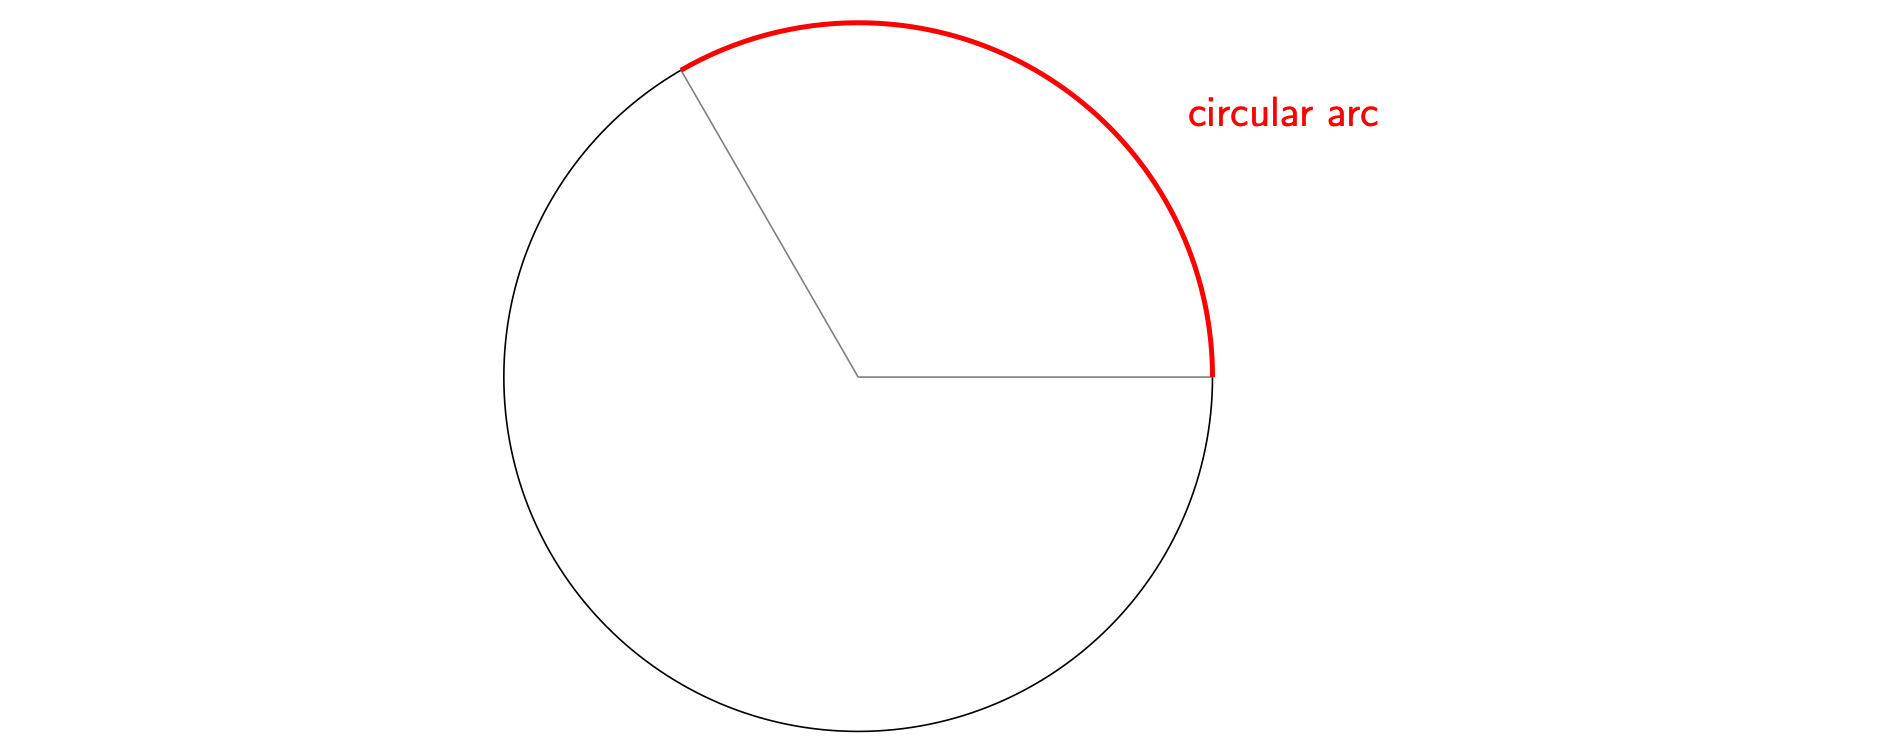
\includegraphics[width=1.5\textwidth,height=\textheight]{./FiguresPNG/radians-circular-arc.png}\end{minipage}%
\end{tcolorbox}

\begin{tcolorbox}[enhanced jigsaw, coltitle=black, rightrule=.15mm, left=2mm, colbacktitle=quarto-callout-note-color!10!white, breakable, arc=.35mm, bottomrule=.15mm, bottomtitle=1mm, toptitle=1mm, title=\textcolor{quarto-callout-note-color}{\faInfo}\hspace{0.5em}{Definition of a circular sector}, colback=white, leftrule=.75mm, colframe=quarto-callout-note-color-frame, toprule=.15mm, titlerule=0mm, opacityback=0, opacitybacktitle=0.6]
Pick two different points on a circle and draw a two lines between them
and the centre. The area between these two lines and an arc between the
points is called a \textbf{circular sector}, but we usually abbreviate
this to just \textbf{sector}.
\end{tcolorbox}

\begin{tcolorbox}[enhanced jigsaw, coltitle=black, rightrule=.15mm, left=2mm, colbacktitle=quarto-callout-note-color!10!white, breakable, arc=.35mm, bottomrule=.15mm, bottomtitle=1mm, toptitle=1mm, title=\textcolor{quarto-callout-note-color}{\faInfo}\hspace{0.5em}{Example 2}, colback=white, leftrule=.75mm, colframe=quarto-callout-note-color-frame, toprule=.15mm, titlerule=0mm, opacityback=0, opacitybacktitle=0.6]
This is an example of a sector.
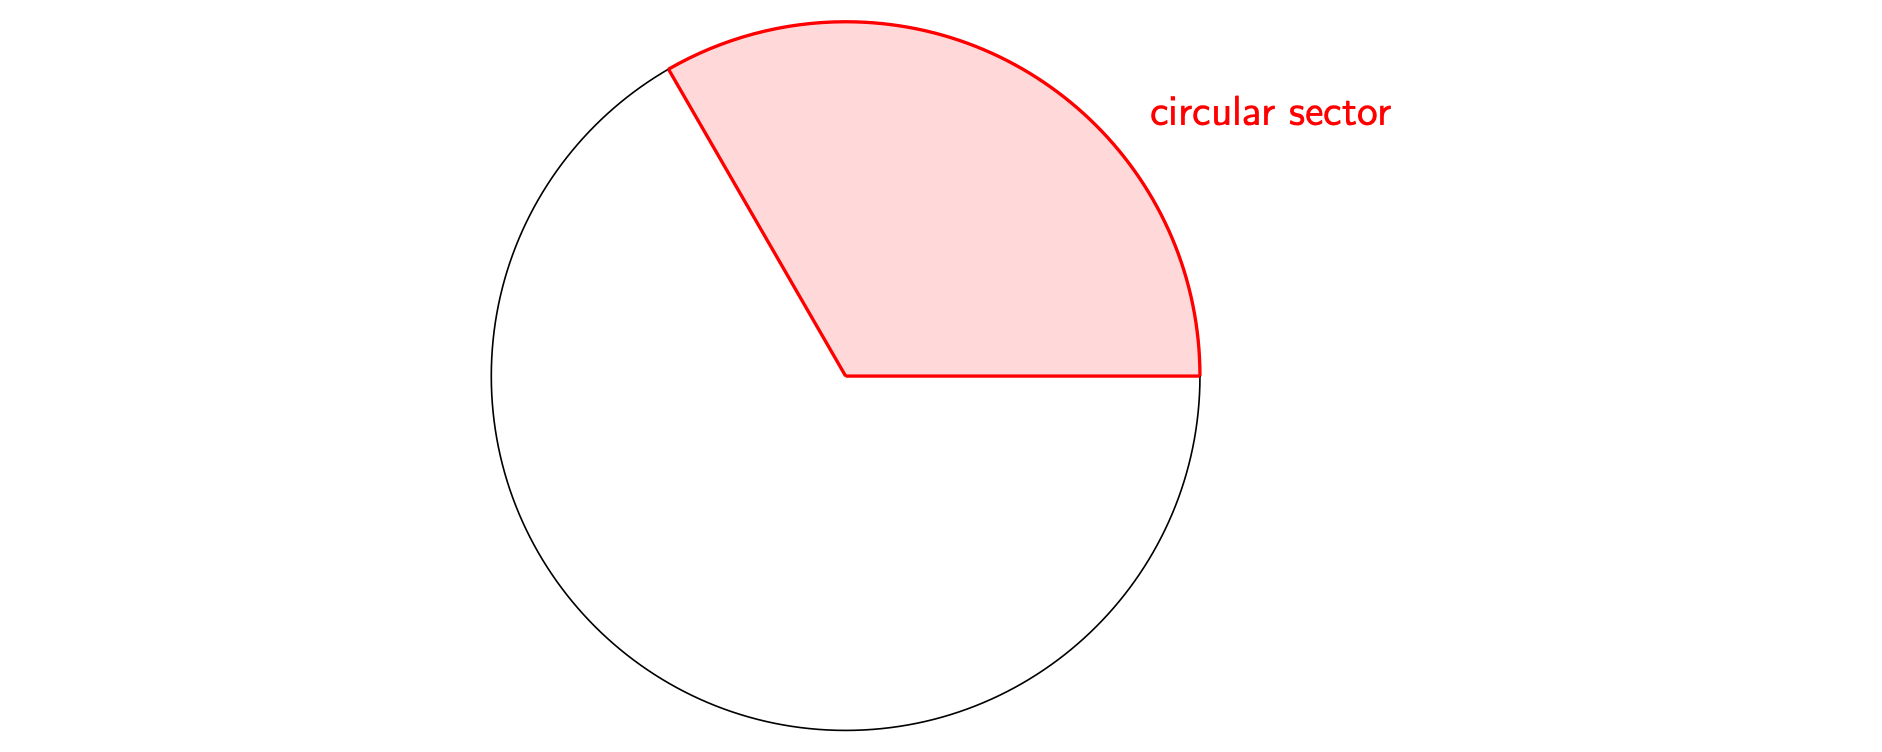
\includegraphics[width=1.5\textwidth,height=\textheight]{./FiguresPNG/radians-circular-sector.png}
\end{tcolorbox}

You can now begin to precisely explain the relationship between radians
and circles!

Pick any two points on a circle such that the length of the arc between
them is equal to the radius of the circle and draw straight lines
between these points and the centre. The angle between these two lines
at the centre is \(1\) rad. A precise way to say this is:

\begin{tcolorbox}[enhanced jigsaw, coltitle=black, rightrule=.15mm, left=2mm, colbacktitle=quarto-callout-note-color!10!white, breakable, arc=.35mm, bottomrule=.15mm, bottomtitle=1mm, toptitle=1mm, title=\textcolor{quarto-callout-note-color}{\faInfo}\hspace{0.5em}{Definition of a radian}, colback=white, leftrule=.75mm, colframe=quarto-callout-note-color-frame, toprule=.15mm, titlerule=0mm, opacityback=0, opacitybacktitle=0.6]
A \textbf{radian} is the angle subtended at the centre of a circle by an
arc that is equal in length to the radius.
\end{tcolorbox}

\begin{tcolorbox}[enhanced jigsaw, coltitle=black, rightrule=.15mm, left=2mm, colbacktitle=quarto-callout-tip-color!10!white, breakable, arc=.35mm, bottomrule=.15mm, bottomtitle=1mm, toptitle=1mm, title=\textcolor{quarto-callout-tip-color}{\faLightbulb}\hspace{0.5em}{Tip}, colback=white, leftrule=.75mm, colframe=quarto-callout-tip-color-frame, toprule=.15mm, titlerule=0mm, opacityback=0, opacitybacktitle=0.6]
The size of the circle doesn't change the value of \(1\) rad - it's the
same in any circle.
\end{tcolorbox}

\begin{figure}

{\centering 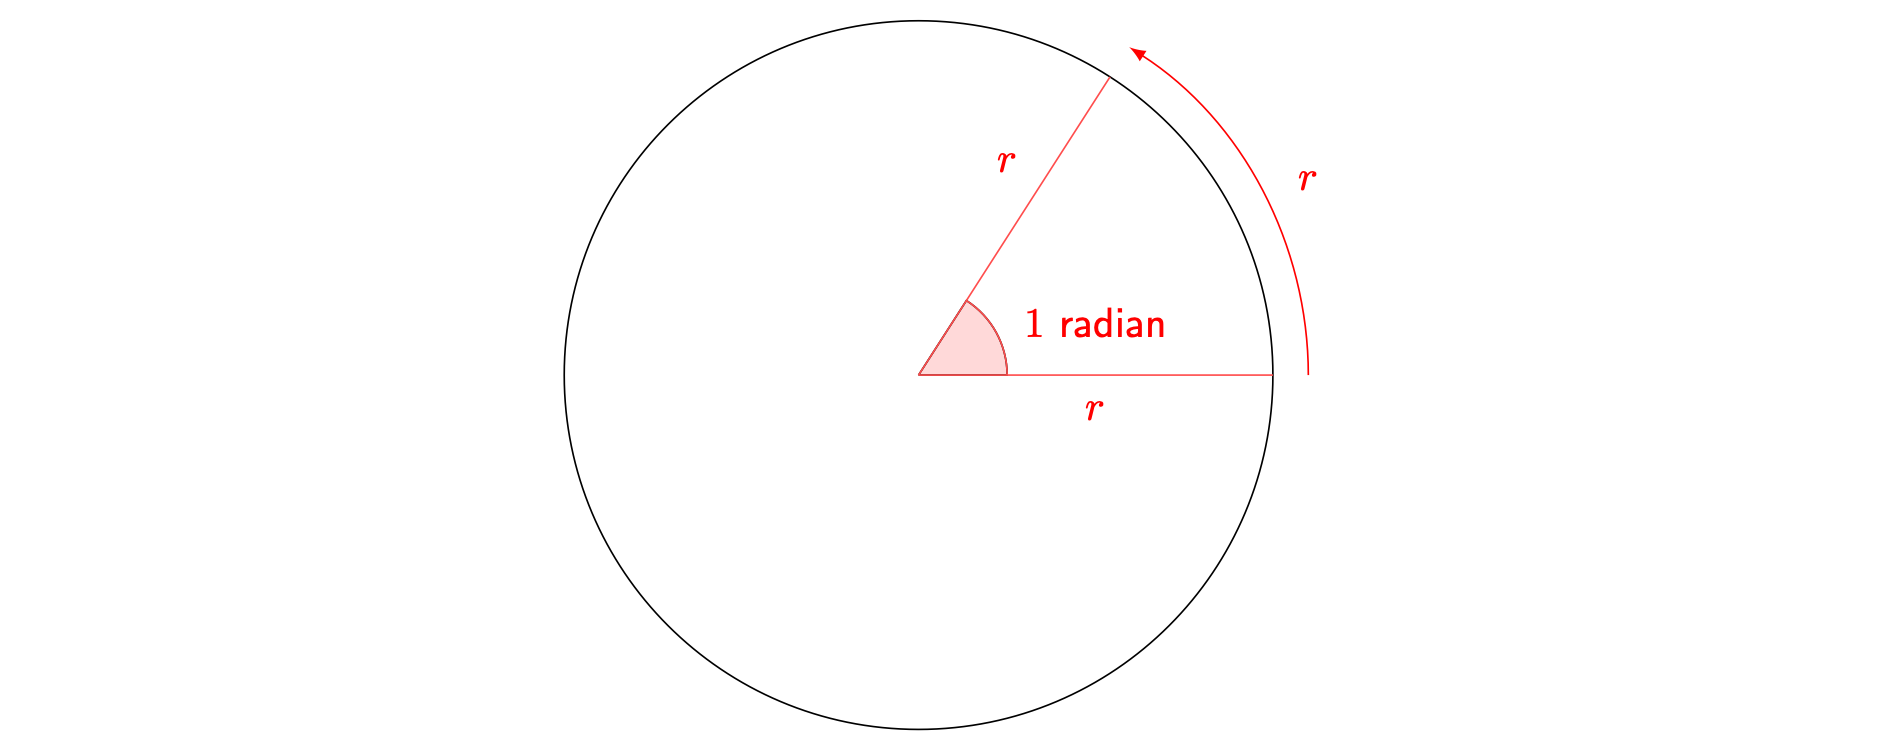
\includegraphics[width=1.5\textwidth,height=\textheight]{./FiguresPNG/radians-radian.png}

}

\caption{A visual representation of a radian.}

\end{figure}

Now, you can get the number of radians in a full circle. The well-known
equation \(c = 2 \pi r\), where \(c\) is the circumference of a circle
and \(r\) the radius, tells you that you can fit sectors with arc length
\(r\) side by side into the circle \(2\pi\) times. Since each of these
sectors has an angle of \(1\) rad at the centre, it follows that there
are \(2\pi\) radians in the whole circle.

\begin{figure}

{\centering 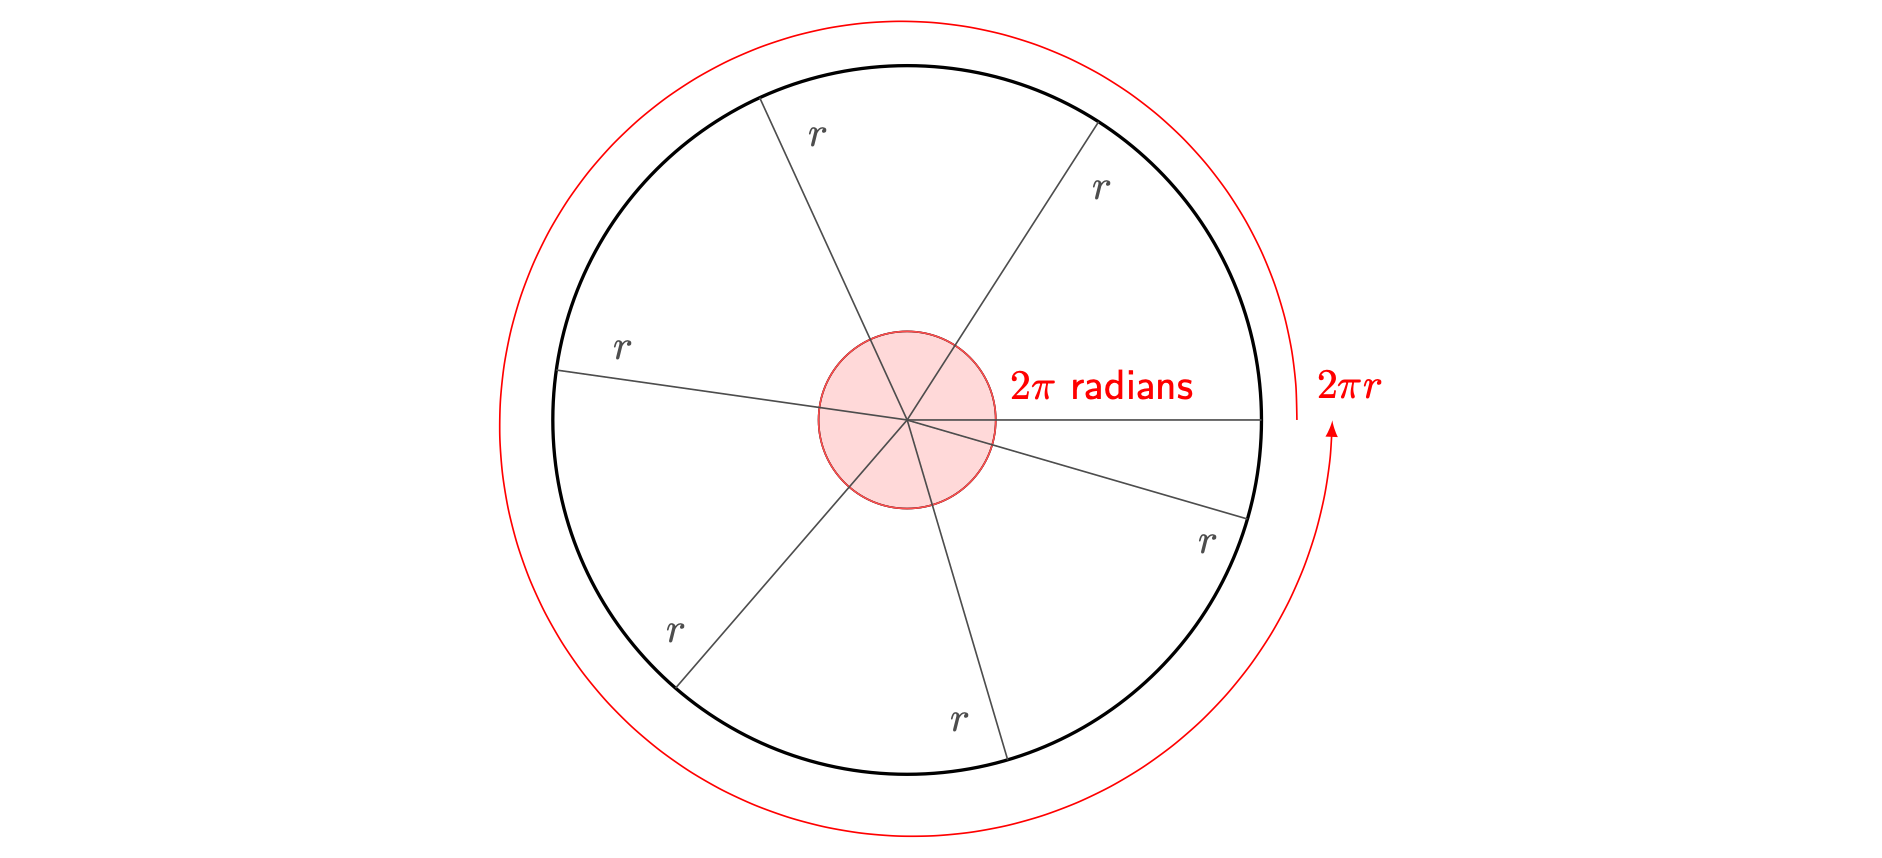
\includegraphics[width=1.5\textwidth,height=\textheight]{./FiguresPNG/radians-circle-divided.png}

}

\caption{A circle divided by sectors with arc length equal to the
radius.}

\end{figure}

\hypertarget{converting-between-radians-and-degrees}{%
\subsection{Converting between Radians and
Degrees}\label{converting-between-radians-and-degrees}}

The process for converting from Radians to Degrees and from Degrees to
Radians are direct opposites.

\hypertarget{converting-from-degrees-to-radians}{%
\subsubsection{Converting from Degrees to
Radians}\label{converting-from-degrees-to-radians}}

Starting from an angle in Degrees.

\begin{itemize}
\tightlist
\item
  Multiply the angle in Degrees by \(\pi\)
\item
  Divide the result by 180
\end{itemize}

Your angle is now in Radians.

\textbf{Remember to simplify fractions}

\hypertarget{example-1-1}{%
\paragraph{Example 1}\label{example-1-1}}

You are given the angle \(180\textdegree\) to convert to Radians.

\begin{itemize}
\tightlist
\item
  Multipying by \(\pi\) gives \(180\pi\)
\item
  Dividing by 180 gives \(\pi\)
\end{itemize}

This means that \(180\textdegree\) is equal to \(\pi\) rad.

\hypertarget{example-2-1}{%
\paragraph{Example 2}\label{example-2-1}}

You are given the angle \(45\textdegree\) to convert to Radians.

\begin{itemize}
\tightlist
\item
  Multiplying by \(\pi\) gives \(45\pi\)
\item
  Dividing by 180 gives \(\frac{\pi}{4}\)
\end{itemize}

This means that \(45\textdegree\) is equal to \(\frac{\pi}{4}\) rad.

\hypertarget{converting-from-radians-to-degrees}{%
\subsubsection{Converting from Radians to
Degrees}\label{converting-from-radians-to-degrees}}

Starting from an angle in Radians.

\begin{itemize}
\tightlist
\item
  Multiply the angle in Radians by 180
\item
  Divide the result by \(\pi\)
\end{itemize}

Your angle is now in Degrees.

\hypertarget{example-3}{%
\paragraph{Example 3}\label{example-3}}

You are given the angle \(\pi\) rad to convert to Degrees.

\begin{itemize}
\tightlist
\item
  Multiplying by 180 gives \(180\pi\)
\item
  Dividing the result by \(\pi\) gives 180
\end{itemize}

This means that \(\pi\) rad is equal to \(180\textdegree\).

\hypertarget{example-4}{%
\paragraph{Example 4}\label{example-4}}

You are given the angle \(\frac{\pi}{4}\) rad to convert to degrees

\begin{itemize}
\tightlist
\item
  Multiplying by 180 gives \(45\pi\)
\item
  Dividing the result by \(\pi\) gives 45
\end{itemize}

This means that \(\frac{\pi}{4}\) rad is equal to \(45\textdegree\).

\hypertarget{useful-conversions-to-know}{%
\subsection*{Useful conversions to
know}\label{useful-conversions-to-know}}
\addcontentsline{toc}{subsection}{Useful conversions to know}

Here is a table of useful conversions of degrees to radians that come up
often:

\begin{longtable}[]{@{}cc@{}}
\toprule()
Degrees (\(\textdegree\)) & Radians (\(\textrm{rad}\)) \\
\midrule()
\endhead
\(360\) & \(2 \pi\) \\
\(210\) & \(\frac{7\pi}{6}\) \\
\(180\) & \(\pi\) \\
\(120\) & \(\frac{2\pi}{3}\) \\
\(90\) & \(\frac{\pi}{2}\) \\
\(60\) & \(\frac{\pi}{3}\) \\
\(45\) & \(\frac{\pi}{4}\) \\
\(30\) & \(\frac{\pi}{6}\) \\
\bottomrule()
\end{longtable}

\hypertarget{arc-length-and-sector-area}{%
\subsection{Arc Length and Sector
Area}\label{arc-length-and-sector-area}}

If you have two straight lines from the centre of a circle to the
circumference and know the angle, in radians, between these lines at the
centre, then you can calculate the length of the arc between these
lines.

\begin{tcolorbox}[enhanced jigsaw, coltitle=black, rightrule=.15mm, left=2mm, colbacktitle=quarto-callout-note-color!10!white, breakable, arc=.35mm, bottomrule=.15mm, bottomtitle=1mm, toptitle=1mm, title=\textcolor{quarto-callout-note-color}{\faInfo}\hspace{0.5em}{Equation for arc length}, colback=white, leftrule=.75mm, colframe=quarto-callout-note-color-frame, toprule=.15mm, titlerule=0mm, opacityback=0, opacitybacktitle=0.6]
The length \(s\) of an arc between two points is given by
\(s = r \theta\), where \(r\) is the radius of the circle and \(\theta\)
is the angle, in radians, between the straight lines from the two points
to the centre.
\end{tcolorbox}

To see why this equation holds, convince yourself that this equality is
true (\(c\) is the circumference of the circle):
\[\frac{s}{c} = \frac{\theta}{2\pi}.\] If you substitute \(c = 2\pi r\)
into this equality, you get \[\frac{s}{2\pi r} = \frac{\theta}{2\pi}.\]
Finally, rearranging gives you the equation \[s = r \theta.\]

Similar to arc length, you can get an equation in terms of radians to
calculate the area of a sector.

\begin{tcolorbox}[enhanced jigsaw, coltitle=black, rightrule=.15mm, left=2mm, colbacktitle=quarto-callout-note-color!10!white, breakable, arc=.35mm, bottomrule=.15mm, bottomtitle=1mm, toptitle=1mm, title=\textcolor{quarto-callout-note-color}{\faInfo}\hspace{0.5em}{Equation for sector area}, colback=white, leftrule=.75mm, colframe=quarto-callout-note-color-frame, toprule=.15mm, titlerule=0mm, opacityback=0, opacitybacktitle=0.6]
The area \(A\) of a sector of a circle with radius \(r\) and angle
\(\theta\) at the centre (in radians) is given by
\(A = \frac{1}{2}r^2\theta\).
\end{tcolorbox}

Showing this is true is left to you in the exercises.

\hypertarget{quick-check-problems}{%
\subsection*{Quick check problems}\label{quick-check-problems}}
\addcontentsline{toc}{subsection}{Quick check problems}



\end{document}
